% Design Development 
\chapter{Design Development}
\label{sec-development}

\begin{remark}  \color{blue}
\begin{itemize}\tightlist
\item The design is the protagonist of the story; the design team is only a supporting character. 
\item Focus on results (e.g., key findings, insights, lessons learned), not activity (``We brainstormed extensively and eventually settled on two alternative concepts.'')
\item Use lots of images, and not just photographs: diagrams, schematics, flow charts, CAD renderings, etc. are often much more informative than a photo. In any case, use labels pointing to the features you want the reader to appreciate.
\item Lengthy details (e.g. detailed results of technical benchmarking) should go in an Appendix section, with an explicit forward reference from this section.
\item Be professional: for benchmarking, it's essential to properly cite sources of information and provide credits for any images you are using that you did not generate yourselves.
\item Don't refrain from describing ideas that were briefly pursued and dropped. Explain why they were abandoned. In other circumstances they might be worth picking up again.
\item You can use tools such as Pugh concept selection, function-structure diagrams and design decomposition to organize and clarify your design process \cite{Otto07,OttoWood01,UlrichEppinger95}.
\end{itemize}
\normalcolor 

The remaining text in this section contains of excerpts from the Autodesk 2007-08 Fall document \cite{Autodesk2008Fall}.
\end{remark}

The broad scope of our problem statement allowed the team members to use their imaginations and arrive at creative solutions. We drew from our diverse individual experiences to redefine the problem as we learned more about existing collaborative tools and practices. Throughout the design development process we balanced pushing forward with our current ideas while constantly looking for new directions. 

\begin{figure}[h]
	\begin{center}
		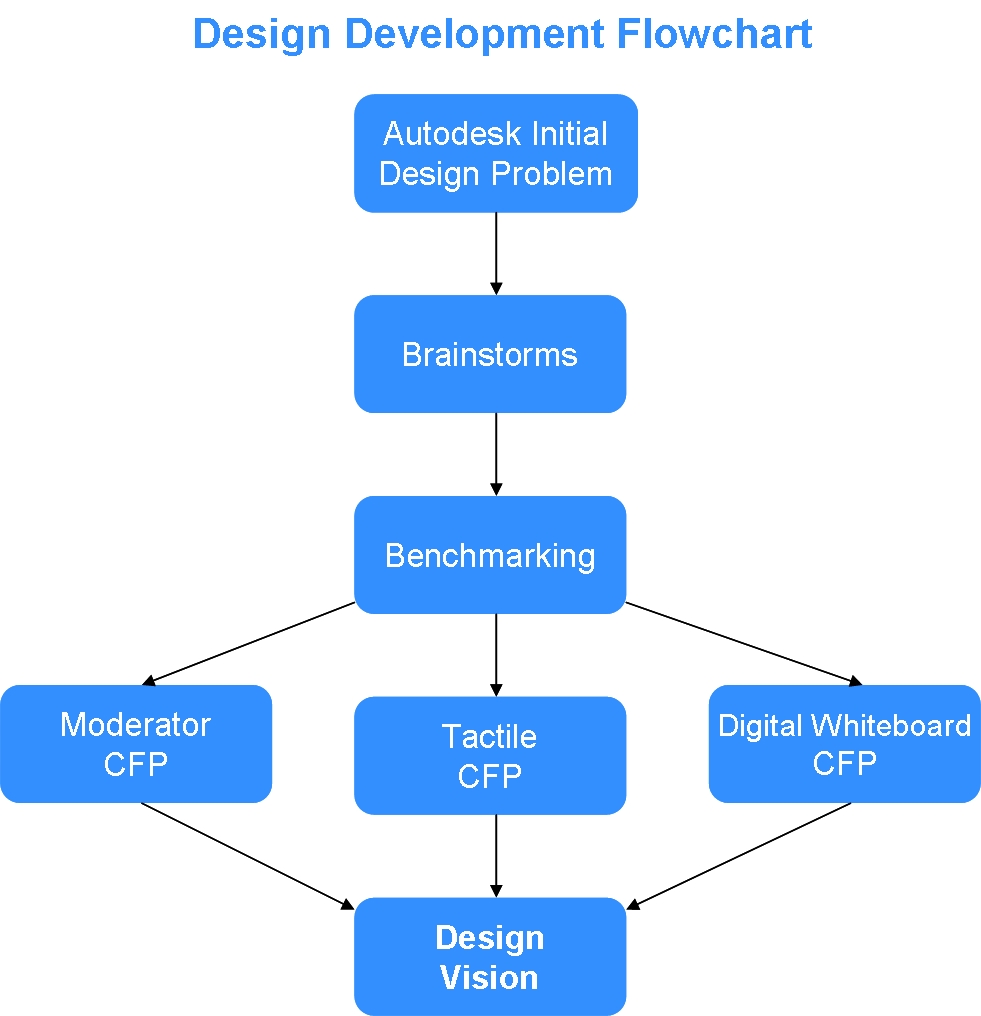
\includegraphics[keepaspectratio, width=4in]{Figures/Ch4/Design_Development_Flowchart.jpg}
	\caption{The design team's development process.}
	\end{center}
	\label{fig:Design_Development_Flowchart}
\end{figure}

\section{Brainstorming}
\label{sec:brainstorm}

	Our experience in brainstorming was unique in that we were observing and studying our own behavior while exploring solutions. We were constantly studying our own triumphs and shortcomings in the hopes of gaining insight into team dynamics. The results of our multiple brainstorms throughout the fall quarter can be into categorized the following categories:

\subsection{Communication}

\begin{figure}[h] 
	\begin{center}
		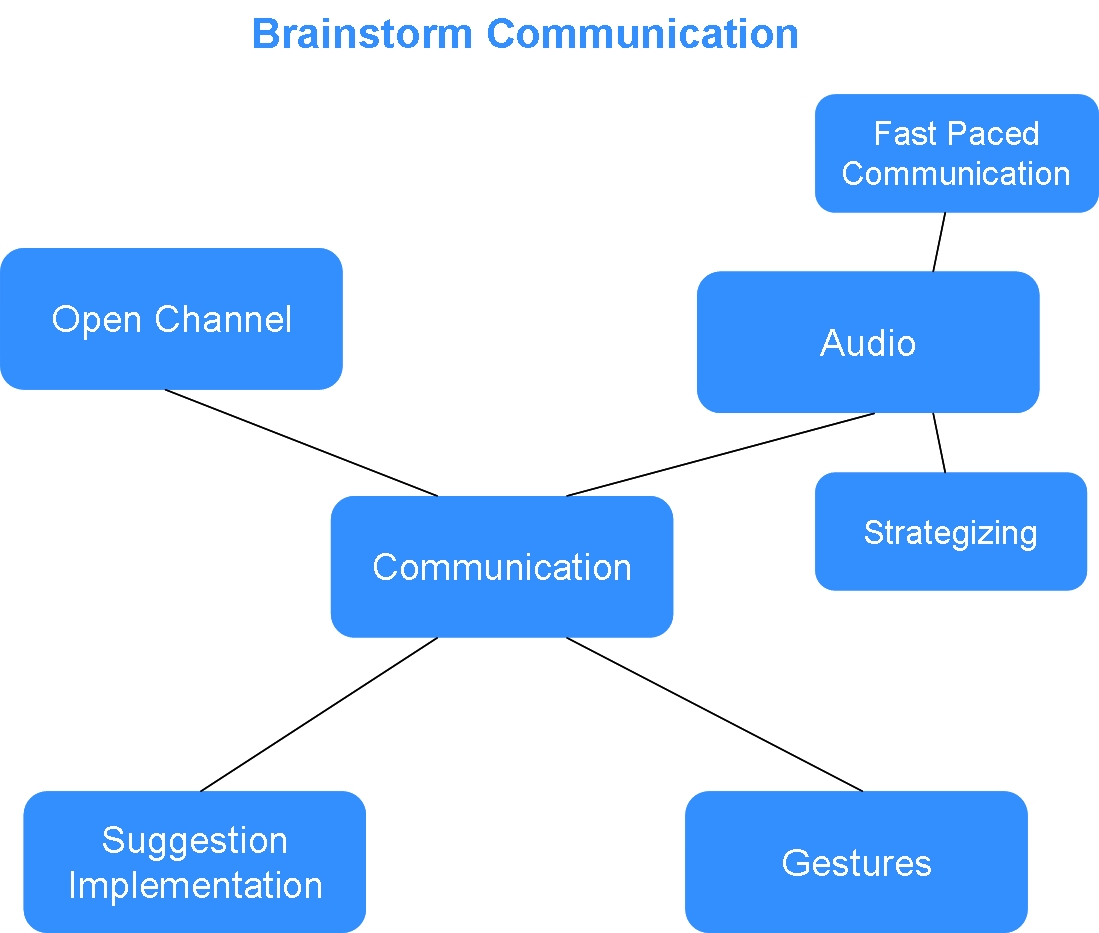
\includegraphics[keepaspectratio, width=3in]{Figures/Ch4/Brainstorm_Communication.jpg}
	\caption{Key components of communication in design meetings}
	\label{fig:Brainstorm_Communication}
	\end{center}
\end{figure}

\begin{itemize} \tightlist 
\item {Open channels}
\item \begin{itemize} \tightlist Audio and video channels are often inundated with information, even if they are not the most effective means to transmit a piece of information. The team learned that messages are most clearly conveyed when they are free from interference. \end{itemize}
\item Integrate suggestions quickly
\item \begin{itemize} \tightlist People can build onto other's ideas immediately, and rapidly change the direction of the conversation. \end{itemize}
\item \textbf{Verbal communication is the most flexible}
\item \begin{itemize} \tightlist The team learned from their experience playing cutting-edge multiplayer videogames that verbal communication was the most relied upon medium during fast and slow paced activities. It's versatility and low-bandwidth warranted future attention. \end{itemize}
\item Gesture
\item \begin{itemize} \tightlist Gesture is frequently used when explaining an idea. Often, the drawings produced do not look at all like the concept being developed, but the act of drawing in and of itself can be like a gesture, showing how something will work, or where it will be placed, and so forth. \end{itemize}
\end{itemize}

\begin{center}
\color{blue}
The rest of this subsection is omitted for brevity
\normalcolor
\end{center}

Some key realizations from the brainstorming phase were that social factors and communication shortcomings had alot of opportunity for development. We decided to give special attention to social benchmarking in addition to our technological research.

\section{Research and Benchmarking}
	The team's research and benchmarking efforts were focused on three major categories: human-machine interfaces and input devices, social dynamics, and communication. The methods the team utilized to research items in these three main categories  included trying out hardware, drawing on previous experience, participating in improv exercises, researching existing solutions, and speaking to experts from design, neuroscience, and computer science.
	
\subsection{The Nintendo Wii \textregistered - Accelerometer-based input)}

\begin{figure}[h] 
\centering
		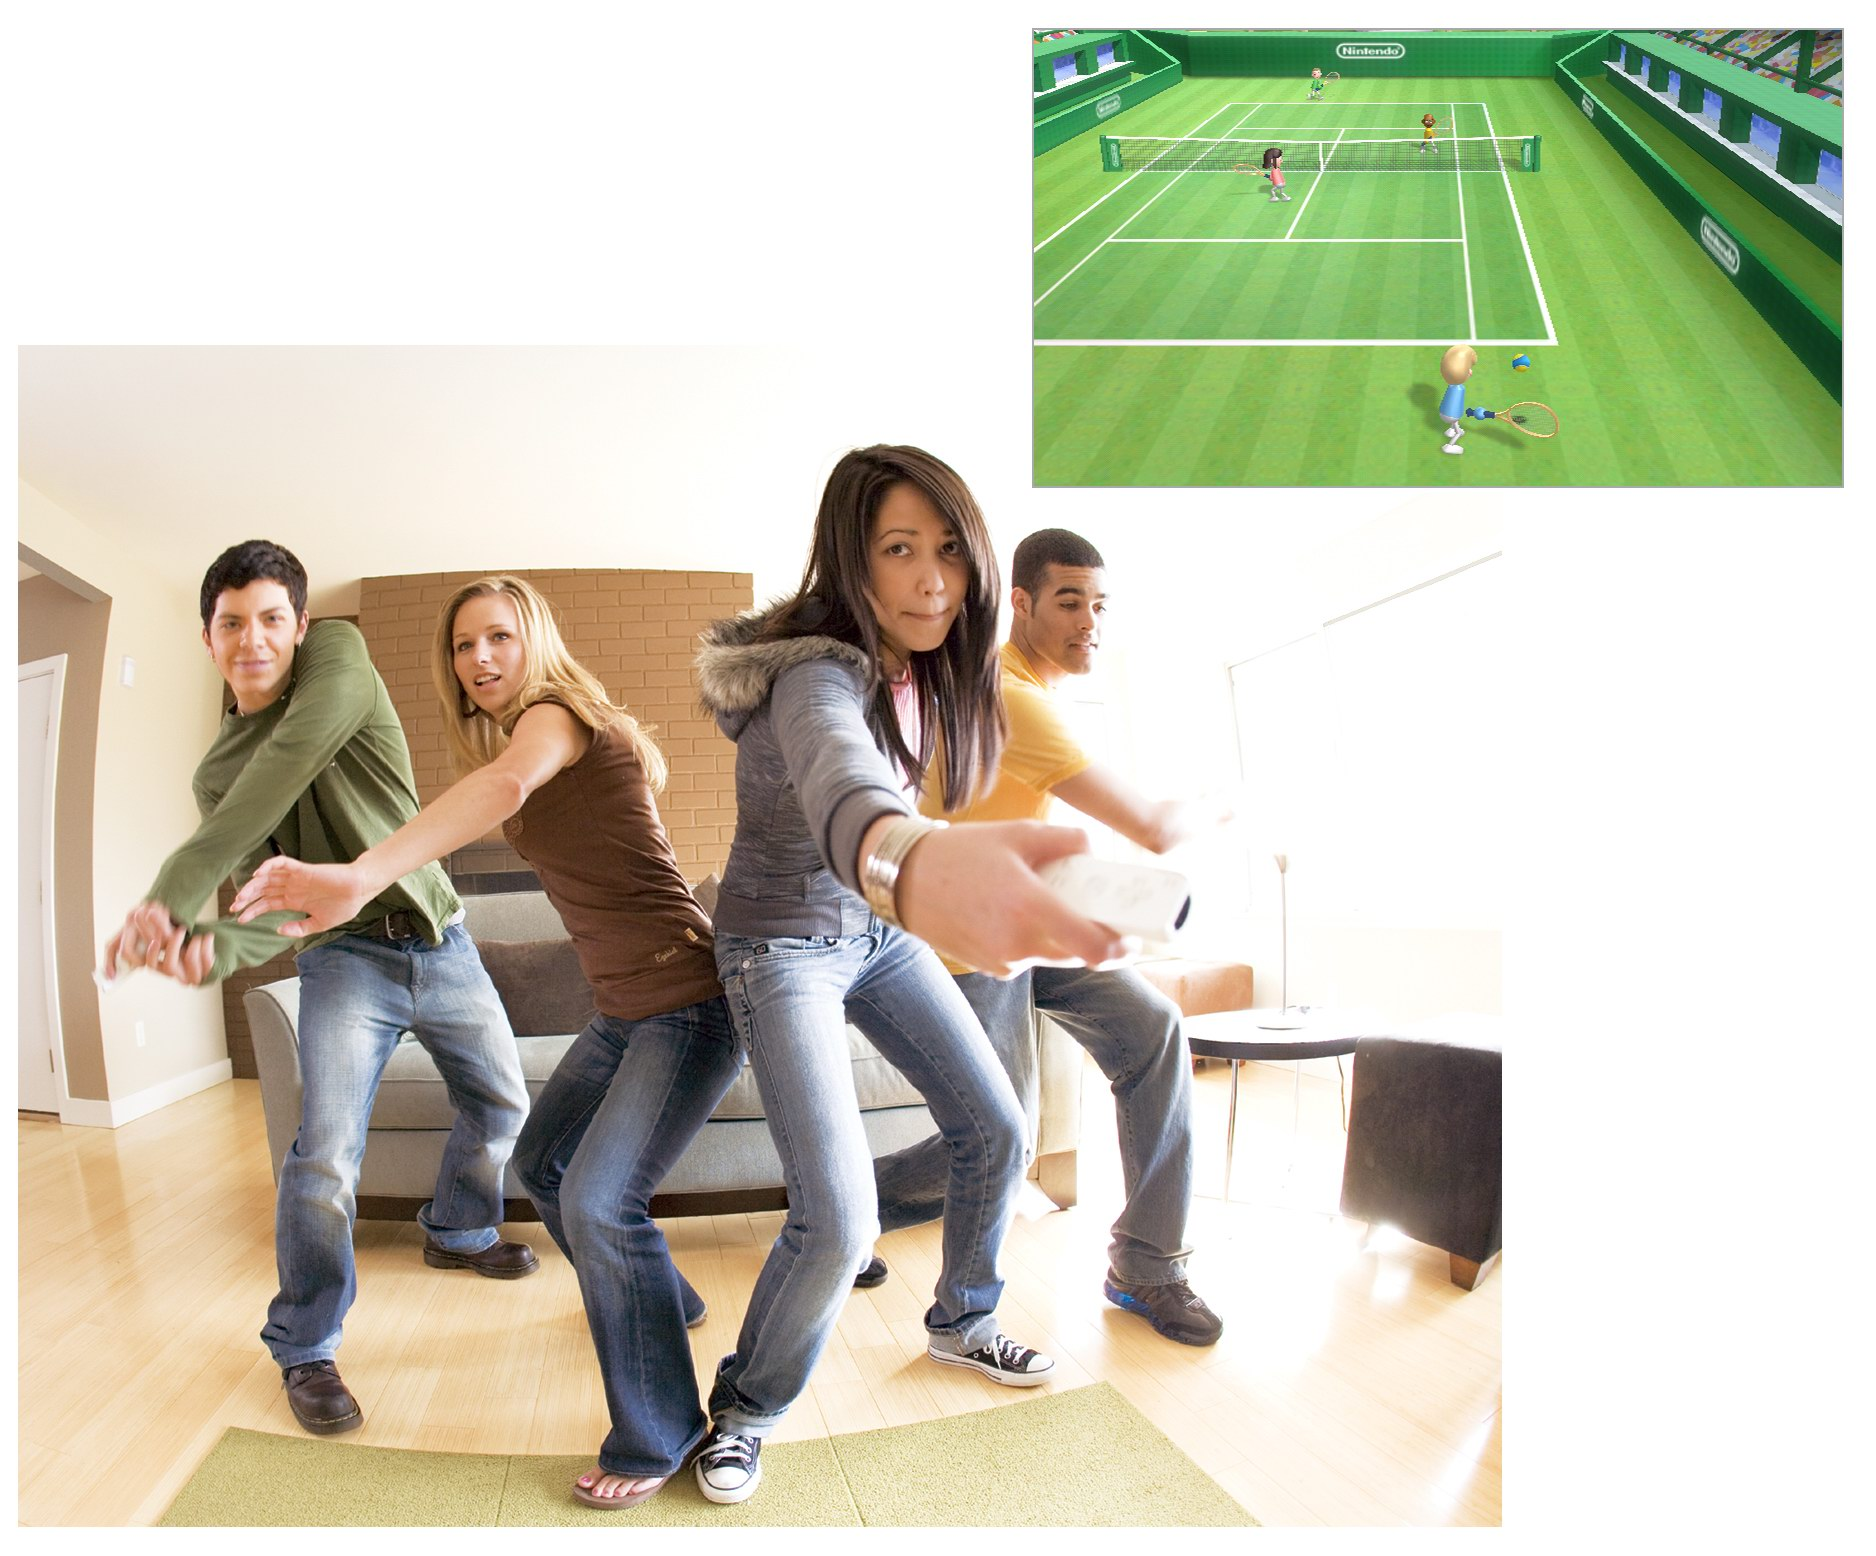
\includegraphics[keepaspectratio, width=4in]{Figures/Ch4/Wii.jpg}
%Note the use of a short caption tag for the list of figures.
	\caption[Nintento Wii]{People playing Wii Sports on the the Nintendo Wii \textregistered.
	\color{blue}Ideally there would be a citation to the URL this photo came from\normalcolor. }
\end{figure}

	The team investigated some unconventional means for data input. Gesture-based input devices like the Nintendo Wii controller offer the possibility of an intuitive, and compelling way to interact with someone at distance via digital means.  For navigating through Windows or other applications, the team found the Wii to be  more challenging than a conventional mouse.  Accelerometers are adept at capturing large motions rather than precision pointing and would need to be utilized as such. Potential applications could be for interfacing with avatars or tactile feedback systems. The Wii controller could be used as a gesture-based communication device to control a personal avatar or send and receive tactile messages.
	
\noindent \textbf {Key lessons learned}
\begin{itemize} \tightlist 
\item Accelerometer based input devices could be used in gesture-based or tactile communication, but do not fare well in precision pointing.
\item Gesture-based interfaces generate excitement. People want to use input devices that respond to gesture. 
\end{itemize}

\subsection{CyberGlove \textregistered}

\begin{figure}[h] 
\centering
		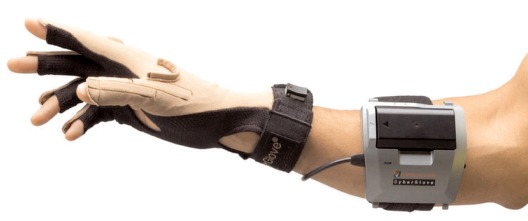
\includegraphics[keepaspectratio, width=4in]{Figures/Ch4/CyberGlove.jpg}	
%Note the use of a short caption tag for the list of figures.
	\caption[Cyberglove]{CyberGlove \textregistered gesture-based input device. \color{blue}Ideally there would be a citation to the URL this photo came from\normalcolor.}
\end{figure}

\begin{center}
\color{blue}
The rest of this subsection is omitted for brevity
\normalcolor
\end{center}

\subsection{EEG and Participation Monitor}

\begin{figure}[h] 
\centering
		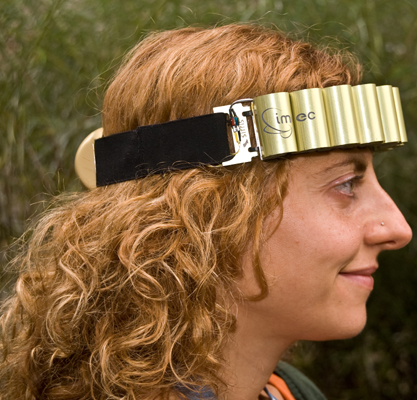
\includegraphics[keepaspectratio, width=3in]{Figures/Ch4/EEG.jpg}
	\caption[Wireless EEG]{Example of the first available wireless EEG tool, made by IMEC. \color{blue}Ideally there would be a citation to the URL this photo came from\normalcolor.}
\end{figure}

	The team met with Alicia Warlick, a researcher in the Stanford Neuroscience Department, and her research in monitoring brainwaves. We discussed the possibility of monitoring whether meeting participants were actively paying attention by using an EEG. This is a method for measuring the activity level of the brain. There is opportunity to use this as a metric for testing our final product, or potentially in the product itself as a means to collect data on user participation level.

\noindent \textbf{Key lesson learned}
\begin{itemize} \tightlist
\item  Electrodes could be placed on the users forehead and scalp to measure EEG readings, which conveys information about whether someone is engaged in what they are doing, or if they are withdrawn.
\end{itemize}

\begin{center}
\color{blue}
The rest of this subsection is omitted for brevity
\normalcolor
\end{center}

\section{Critical Function Prototypes (CFP)}
	The initial benchmarking phase lead the team to realize that there were three major challenges to solve: bridging the proximity gap, moderating brainstorming, and conveying and recording ideas. The team decided to tackle all three of these major challenges and designed four CFPs in an attempt to solve, or at least start answering some of, the questions these challenges brought up. 

\subsection{Tactile CFP}
	
\subsubsection{Tactile CFP Concept Development}

The team wanted to come up with a creative solution that would enhance distance communication. Although we identified software having an important role in our solution, we wanted to try to design something physical. We had to answer these questions that were raised after the benchmarking process:
\begin{itemize} \tightlist
\item How can we simulate proximity for remote meetings?
\item How can we implement action-event control?
\item What senses can we stimulate that aren't normally used?
\item What is a low bandwidth solution?
\end{itemize}

	The team decided that building a tactile messaging system would solve all four of the aforementioned questions. Tactile messages could replace common interpersonal interaction found in same room meetings. It is normal to welcome each other with a  handshake, make eye contact throughout a meeting, smile at each other, and give high-fives to congratulate others. These occurrences are all absent from distance meetings. A tactile message corresponding to each of these gestures would allow users similar opportunity to communicate as if they were sharing the same physical meeting room.
	
	The team learned that immersive activities like videogames take advantage of action-event control to offer users a seamless means to interact with their environment. A tactile message could quickly be sent over an open channel and pressing the �on� button would instantly message the recipient.
	
	Out of the five senses (sight, hearing, taste, touch, and smell), sight and hearing are the most relied upon during meetings. The team considered possibilities in taste and smell messaging but continued with touch, since delivery of tactile messaging was much more straightforward. Since conventional distance meetings only send and receive auditory and visual information, tactile messages would be distinct and easy to identify. The team believed that tactile messages (high, low, or off) would be low bandwidth.

	\begin{figure}[h] 
\centering
		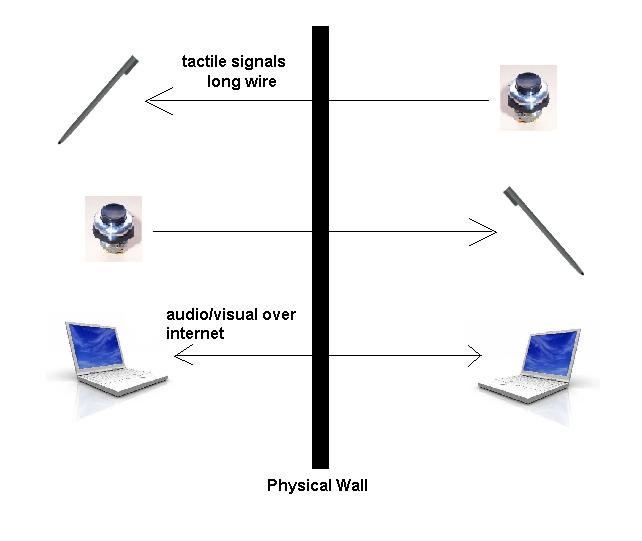
\includegraphics[keepaspectratio, width=4in]{Figures/Ch4/tactileCFPschematic.jpg}
	\caption{The team's whiteboard during a brainstorm session}
\end{figure}

	The team wanted to test the effectiveness of tactile messaging and decided against a TCP/IP protocol that sent messages between Stanford and PUJ. The code to write such a protocol was extant and it was unnecessary to include it in our prototype. The team simplified the setup and created two stations separated by physical barriers (a wall and 50' of distance), to simulate a distance meeting. Each station would have a vibrating tactile device for each seated participant at that station and a high/low button assembly to activate the vibrating tactile device for each participant at the other station. Initially the devices were supposed to operate as ''on'' or ''off.'' The team decided that having more variability in the operating speeds of the motors would increase the number of different messages that could be sent, and added a high and low voltage button (1.2V and 0.6V).
	We were curious to see if effective communication could take place if a distant colleague could see what sketches his distant colleague was drawing. To test this, we used webcams to send live video of what the participants drew on their drawing pads to the other stations.

\subsubsection{What is critical about this CFP?}
	The team identified these questions as critical before testing:
\begin{enumerate} \tightlist
\item Can it create immersion?
\item Does it improve upon existing communication tools?
\item Is it easy to understand?
\item Is it intuitive?
\item When should it be used?
\end{enumerate}

\begin{figure}[h] 
	\begin{center}
		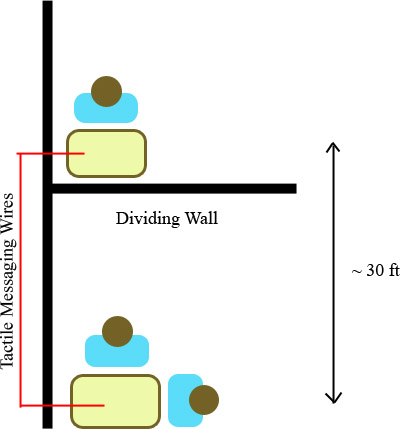
\includegraphics[width=3in]{Figures/Ch4/tactile_seating.jpg}
	\caption{The orientation of the two tactile messaging stations.}
	\end{center}
\end{figure}

%A transcript of the meeting with tactile feedback is available in Appendix \ref{sec:tactiletranscript}.

\subsubsection{Lessons Learned}

	Tactile sensation is an effective means of communicating contextual information. The messaging system delivered instant vibration between the two stations, helping preserve the flow of conversation without impeding it. Using the vibrations to alert the other users that you wanted to say something was a good way to make comments at the precise time you intended. The tactile devices were \textbf{easy to use} and the participants were encouraged to use them as they saw fit. We noticed that \textbf{vibrations were used most frequently to add emphasis} � to accompany laughter, to confirm agreement, offer praise for a good idea � and to interrupt the speaker. Interruptions consisted of calls for clarification on a point raised or disagreement with an opinion. Interrupting someone who is speaking can cause the speaker to lose his train of thought or become otherwise agitated. We noticed that \textbf{users preferred to send low speed vibrations} as a gentle interruption as a first attempt to get the speaker's attention. If the first few low speed vibrations did not stop the speaker, the high speed vibrations could be sent, and these usually registered right away. We observed that users reserved high speed vibrations for urgent or important messages. 
	
	
	The signals were mostly easy to detect, but it was \textbf{not always clear what those signals were trying to communicate}. Ambiguous or superfluous signals distracted the receiving user from the meeting and the confused user would ask, ''Did you just buzz me?'' or ''�Why did you buzz me?'' These confused questions would stall the meeting for everyone until the sender was revealed and was able to explain what they were trying to communicate. 
	
	Vibrations, however, were easily detectable despite loud side conversations, a party in a neighboring room, and constant distractions from people walking by. We attribute this to the fact that the tactile channel is uncrowded compared to the audio channel. In a loud environment it is difficult to pick out audio communication from Skype. Visual distractions make it difficult to focus on the laptop monitor. The tactile sensation rarely stimulated in a teleconference, thus making the slightest vibration very noticeable. 
	
	We tried two different vibrating interfaces, a vibrating pen and a vibrating wrist patch. The wrist patch was unanimously rejected by the participants because 1) the double stick tape that connected the patch to the user's skin was either too sticky and removed arm hair or not sticky enough after a few uses and would fall off, 2) was tethered to the power supply and restricted movement to the point where the hand with the patch was essentially stationary, 3) vibrations on your wrist are not comfortable, and 4) worry that the patch might give the user an electrical shock. The pen had a practical use, writing, and although the pen was connected to the power supply, the user was not, and the range of motion was adequate enough to write anywhere on the drawing space.
	
	We finally compared the tactile messaging conference to previous experiences with video conferencing and audio conferencing. These results are summarized in Appendix \ref{sec:Appendix1}.
	
		\begin{figure}[h] 
\centering
		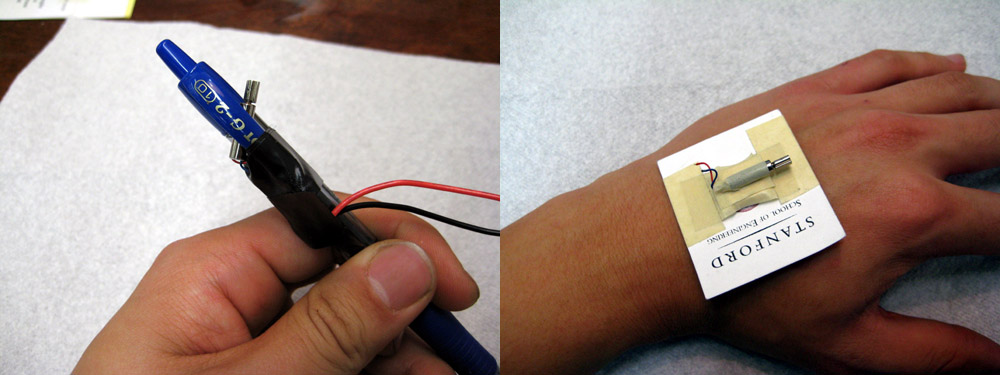
\includegraphics[width=0.8\textwidth]{Figures/Ch4/tactile_motor.jpg}
	\caption[Messaging station wires]{The orientation of the two tactile messaging stations. (Note: the wires connecting the patch to power supply are not in this photo)}
\end{figure}

	The tactile messaging critical function prototype was a success in that it definitively answered all the critical questions we asked ourselves before testing.